\section{Introduction}\label{sec:intro}
Due to the prevelance of large and dirty databases, there is an increasing commercial and research interest
in scalable data cleaning.
Data cleaning often involves humans, whether expert data scientists or the crowd, and it is often infeasible to clean an entire large database. 
To address this problem, two popular design paradigms have emerged, sample-and-clean and progressive data cleaning. 
In the sample-and-clean paradigm, the data scientist ``cleans" a sample of data and she can use this sample of clean data as training examples for a learning-based system (e.g, Coreleone \cite{DBLP:conf/sigmod/GokhaleDDNRSZ14}), data transformation demonstrations (e.g, Wrangler \cite{DBLP:conf/uist/GuoKHH11}), or the estimation of aggregate query results (e.g, SampleClean \cite{wang1999sample}).
In the progressive cleaning paradigm \cite{altowim2014progressive}, the data is progressively cleaned giving the user the best result at the time either to improve accuracy or to work with changing base data \cite{volkovs2014continuous}.

However, depite this interest, large-scale data analytics platforms such as the Spark or Hadoop lack integrated data cleaning frameworks.
Furthermore, existing sample-and-clean and progressive cleaning frameworks only address a subproblem such as extraction or entity resolution.
The problems with dirty data are often very domain and task specific and these limitations make building and maintaining a new data cleaning procedure challenging.
In this demonstration, we present our Spark library \projx which abstracts many of the salient features of these data cleaning frameworks into composable primitives.

\begin{figure}[tup]\label{fig:arch}\vspace{-.5em}
\centering
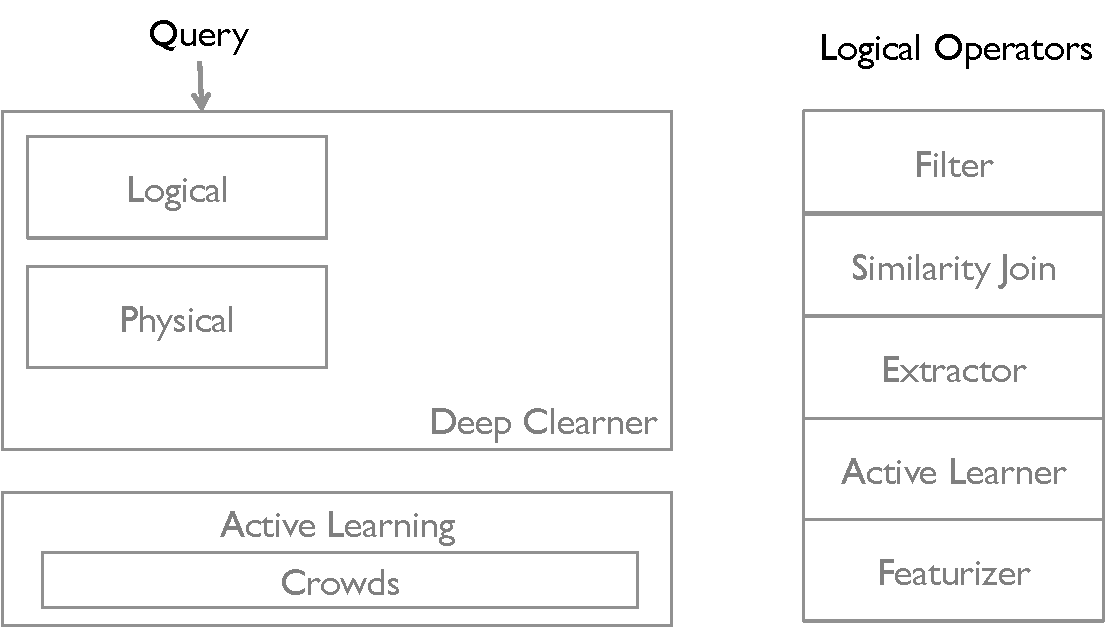
\includegraphics[width=\columnwidth]{figs/architecture.pdf}\vspace{-1em}
\caption{\saqpplus Architecture \label{fig:sample}}

\end{figure}

\projx decomposes data cleaning tasks into three key operators: Extraction, Similarity Join, and Filtering.
These operators can be exectued either in an automated way, with crowdsourcing, or a hybrid.
To this effect, \projx also provides an API for crowdsourcing, fast automated featurization, and active learning.
Finally, \projx provides asynchronous wrappers that allow data cleaning operations to be executed in the background during analytics and an online approximate query processing library to allow for result estimation.
\projx seamlessly integrates with other components in the Spark ecosystem such as SparkSQL \cite{d}, MLBase \cite{d}, and GraphX \cite{d}.

In Figure \ref{fig:sample}, we illustrate the architecture of \projx.
We implement the library as a two layer stack: (1) an API layer that provides composable components that implement the high-level operations, and (2) an execution layer that implements the operators layer either as crowd microtasks or optimized Spark tasks.
The execution layer also has asynchrony and persistence built in to allow for execution of the API layer operations in the background during analytics.

\vspace{0.5em}

\begin{demonstration}[Social Media Analysis]
Analysis of social media, e.g tweets or facebook posts, often requires parsing dirty data.
In this scenario, the VLDB attendees will analyze a real dirty dataset of 1000 tagged political comments with the following schema:
\begin{lstlisting}
Comment(userid, party_affiliation, 
comment_text, tags)
\end{lstlisting}
\textsf{userid} is the primary key of the table, \textsf{party\_affiliation} is string representation of the user's party affiliation (Republican or Democrat), 
\textsf{comment\_text} is the text of the comment, and \textsf{tags} are a delimited string of comment topics.

\begin{figure}[tup]
\centering
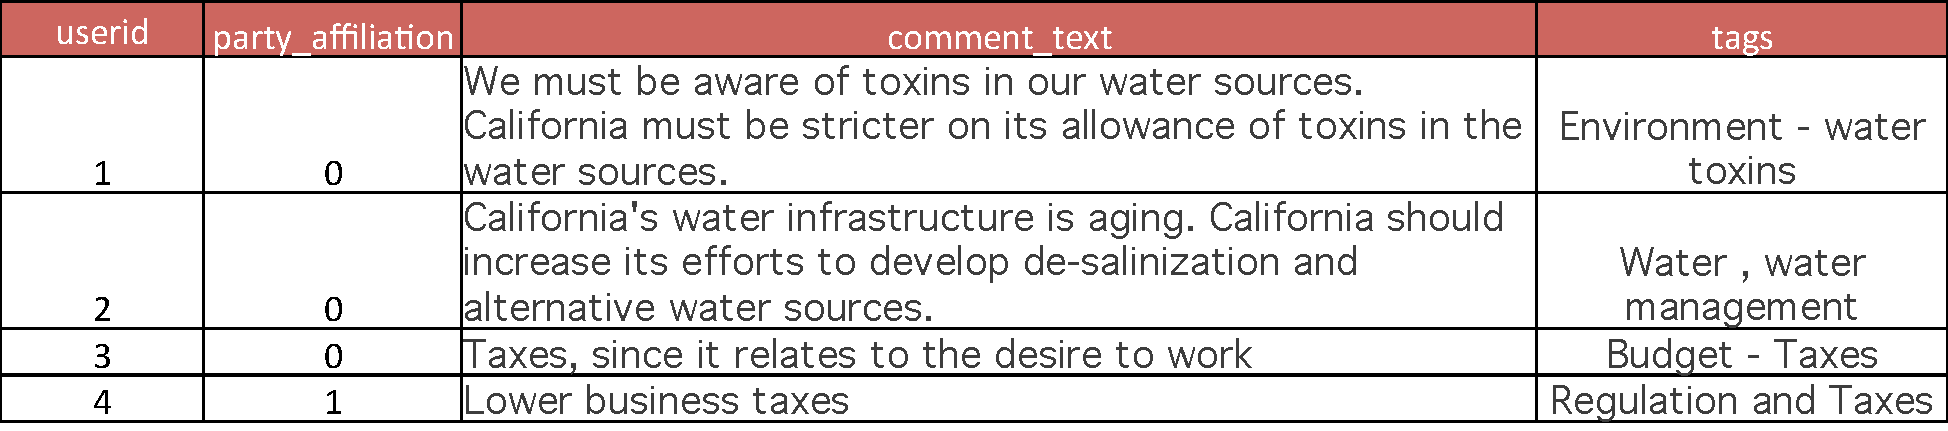
\includegraphics[width=\columnwidth]{figs/dirty-data.pdf}
\caption{ \label{fig:dsample}}\vspace{-.5em}
\end{figure}

The analysis questions are: (1) which topics are the most popular, (2) which topics are the most popular among Democrats/Republicans, and (3) how well can we predict political affiliation from the listed topics.
%We want to know whether Republicans write more comments about fiscal issues than Democrats.
The challenge is that the \textsf{tags} attribute is inconsistent in its representation.
In Figure \ref{fig:dsample}, we show an excerpt from the dataset.
\textsf{tags} is inconsistently delimited and furthermore the delimited topics are inconsistently represented.
The cleaning of this dataset requires a combination of Extraction and Deduplication cleaning operations.

The key benefit of our system is that we can combine both automated and crowd-based techniques.
We will provide demo participants two variants of each operation.
For Extraction, we will allow the participant to either demonstrate example extractions on a sample and learn a general extraction policy; or we 
they can simply specify a set of delimiters.
For Deduplication, we will either do an automated Edit Distance based merging of similar tags; or in an Active Learning loop interactively request help from the user on difficult pairs of tags.
As the dataset get increasingly clean, we will plot the progression of the results to our analysis questions.
\end{demonstration}

\vspace{1em}

In summary, this demo illustrates the composability of data cleaning pipelines written with \projx, how the clean data can be seamless integrated with the Spark ecosystem, and the benefits of crowd-machine hybrid cleaning techniques.
In this demonstration proposal, we describe our framework from the bottom up.
First, we will describe how the three key operators, Extraction, Similarity Join, and Filtering, can describe a wide variety of data cleaning tasks. 
Then, we will describe the execution layer of these operators.
Finally, we will characterize the performance of our system and preview the demo interface.





